%%%%%%%%%%%%%%%%%%%%%%%%%%%%%%%%%%%%%%%%%%%%%%%%%%%%%%%%%%%%%%%%%%%%%%%%%%%%%%%%%%%
% 			Facultad de Ciencias, UAEM.	
% 
%	Alumno: 				Emanuel García Perez
%	Asginatura:				Estructura de Datos
%	Tema:					"Listas Dinamicas"
%
%%%%%%%%%%%%%%%%%%%%%%%%%%%%%%%%%%%%%%%%%%%%%%%%%%%%%%%%%%%%%%%%%%%%%%%%%%%%%%%%%%%


\documentclass{beamer}

\usepackage[utf8]{inputenc}
\usepackage[spanish,activeacute]{babel}
\usepackage[latin1]{inputenc}
\usepackage{beamerthemeshadow}
\usepackage{graphicx}
\usepackage{listings}

\title{\textbf{LISTAS DINÁMICAS}}
\author{Emanuel García Pérez}
\date{\today}

\begin{document}

\frame[allowframebreaks]{\titlepage}
\section[Contenidos]{}
\frame{
\transdissolve[duration=0.2]
\tableofcontents
}


\section{Listas Enlazadas(Estructuras Ligadas)}
\frame
{
\transdissolve[duration=0.2]
\frametitle{?`Qué es una lista enlazada?}
Una lista enlazada es una colección o secuencia de elementos dispuestos uno detrás de otro, en la que cada elemento se conecta al siguiente elemento por medio un \textbf{“enlace”} o \textbf{“puntero”}.
\begin{figure}
  \centering
    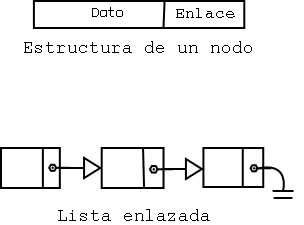
\includegraphics[width=0.5\textwidth]{lista_enlazada.png}
  \label{fig:ejemplo}
\end{figure}
}

\frame
{
\transdissolve[duration=0.2]
\frametitle{Constitución de una lista enlazada}
La idea básica consiste en construir una lista cuyos elementos llamados nodos se componen de dos partes o campos: el primer campo contiene la \textbf{información} o datos del elemento, y por tanto es de tipo genérico (Dato, TipoElemento, Info), y el segundo campo es un \textbf{puntero} (enlace, conector, siguiente) que apunta al siguiente elemento de la lista.
\begin{figure}
  \centering
    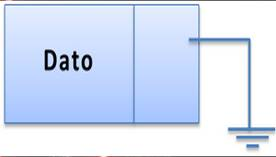
\includegraphics[width=0.5\textwidth]{nodo.jpg}
  \label{fig:ejemplo}
\end{figure}
}

\subsection{Clasificación}
\frame{
\transdissolve[duration=0.2]
\frametitle{Clasificación de listas enlazadas}
\begin{enumerate}
	\item Lista Enlazada Simple
	\item Lista Doblemente Enlazada
	\item Listas Circular Simple
	\item Lista Circular Doblemente Enlazada
\end{enumerate}
}

\frame{
\transdissolve[duration=0.2]
\frametitle{Lista Simple}
\begin{figure}
  \centering
    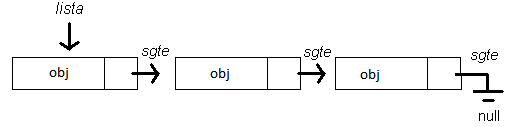
\includegraphics[width=1.0\textwidth]{lista_simple.png}
  \label{fig:ejemplo}
\end{figure}
}
}

\frame{
\transdissolve[duration=0.2]
\frametitle{Lista Doble}
\begin{figure}
  \centering
    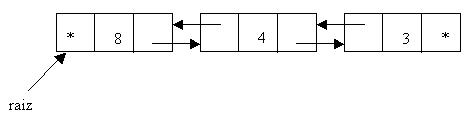
\includegraphics[width=1.0\textwidth]{lista_doble.jpg}
  \label{fig:ejemplo}
\end{figure}
}
}

\frame{
\transdissolve[duration=0.2]
\frametitle{Lista Circular Simple}
\begin{figure}
  \centering
    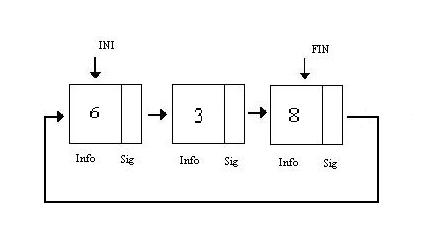
\includegraphics[width=1.0\textwidth]{lista_circular_s.JPG}
  \label{fig:ejemplo}
\end{figure}
}
}

\frame{
\transdissolve[duration=0.2]
\frametitle{Lista Circular Doble}
\begin{figure}
  \centering
    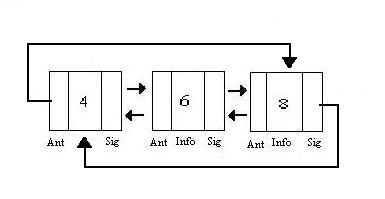
\includegraphics[width=1.0\textwidth]{lista_doble_c.JPG}
  \label{fig:ejemplo}
\end{figure}
}
}

\subsection{Operaciones}
\frame{
\transdissolve[duration=0.2]
\frametitle{Operaciones sobre listas enlazadas}
\begin{itemize}
	\item Inicialización
	\item Insertar elementos
	\begin{itemize}
	\item Al inicio
	\item En medio
	\item Al final
	\end{itemize}
	\item Eliminar elementos
	\begin{itemize}
	\item Al inicio
	\item En medio
	\item Al final
	\end{itemize}
	\item Buscar elementos
	\begin{itemize}
	\item Hacia adelante
	\item Hacia atrás
	\end{itemize}
	\item Recorrer la lista
	\begin{itemize}
	\item Hacia adelante
	\item Hacia atrás
	\end{itemize}
\end{itemize}
}

\section{Aplicaciones de Listas Enlazadas}
\frame{
\transdissolve[duration=0.2]
\frametitle{TDA's}
\begin{itemize}
	\item PILAS
	\item COLAS
	\item Tablas HASH
	\item Arboles
	\item Grafos
\end{itemize}
}

\section{Listas Enlazadas en C}
\subsection{TDA Nodo}
\frame{
\transdissolve[duration=0.2]
\frametitle{Definición del tipo de dato abstracto: Nodo}
\lstinputlisting[language=C]{struct.c}
}

\subsection{Memoria Dinamica}
\frame{
\transdissolve[duration=0.2]
\frametitle{malloc()}
\lstinputlisting[language=C]{memoria.c}
}

\frame{
\transdissolve[duration=0.2]
\frametitle{free()}
\lstinputlisting[language=C]{memoria2.c}
}

\subsection{Punteros y acceso al TAD}
\frame{
\transdissolve[duration=0.2]
\frametitle{Dirección, Indirección y acceso a Miembro.}
\begin{itemize}
\item \&: Operador de dirección, da acceso a la dirección de la variable que estamos referenciando.
\item *: Operador de indirección, 	da acceso al contenido de la variable que estamos referenciando.
\item -$>$: Operador de acceso, nos permite acceder a un miembro determinado de una estructura que esta siendo referenciada a través de punteros.
\end{itemize}
}


\end{document}